\documentclass[12pt, titlepage, oneside]{article}
\usepackage[letterpaper, margin=1in]{geometry}
\usepackage{siunitx, booktabs, amsmath, enumitem, pdfpages, tabularx,caption, graphicx, pgfplots, textcomp}
\usepackage[siunitx]{circuitikz}
\sisetup{detect-weight=true, detect-family=true}
\usepackage{wrapfig}
\usepackage{mathrsfs}
\setlength\parindent{0pt}
\let\oldhat\hat
\let\oldvec\vec
\newcommand{\cross}{\bm{\times}}
\renewcommand{\hat}[1]{\oldhat{\mathbf{#1}}}
\usepackage{bm}
\renewcommand{\vec}[1]{\oldvec{\bm{#1}}}
\renewcommand{\hat}[1]{\oldhat{\bm{#1}}}
\renewcommand{\b}[1]{\textbf{#1}}

\begin{document}
\section*{24.1 Electric Flux}
\noindent\fbox{%
	\parbox{\textwidth}{%
	The product of the magnitude of the electric field and surface area perpendicular to the field is called \textbf{electric flux} $\Phi_E$ [N $\cdot$\si{m^2/C}]
	}
}
\\ \vspace{0.5cm}

\begin{wrapfigure}{r}{0.3\textwidth}
\begin{center}
	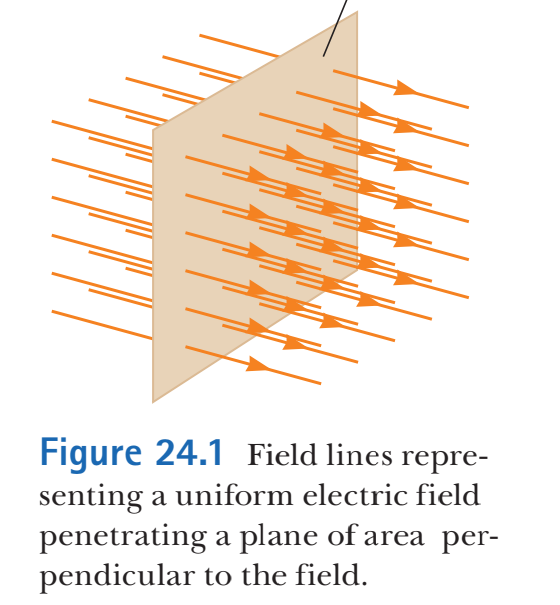
\includegraphics[scale=0.5]{1.png}
\end{center}
\end{wrapfigure}
We notice that since we only care about the field lines perpendicular to the surface, we can find the angle between the field line and a normal vector to the surface. 
\begin{align*}
	\Phi_E = EA_{\perp} = EA \cos \theta
\end{align*}
For maximum value of flux, we would like $\theta = 0^{\circ}$, and for minimum we would like $\theta = 90^{\circ}$\\
Let there be $\vec{A}$ which has magnitude of surface area and has a vector normal to the surface. Now, let us make this area $\vec{A}$ really small to $\Delta \vec{A}$. And let us add each of these small electric fluxes at every area.

\begin{align*}
	\Phi_E \approx \sum \vec{E_i} \cdot \Delta \vec{A_i}
\end{align*}
\noindent\fbox{%
	\parbox{\textwidth}{%
		\textbf{Electric Flux}	
	\begin{align}
		\Phi_E = \int \limits_{\text{Surface}} \vec{E} \cdot d\vec{A}
	\end{align}	
}}
\begin{wrapfigure}{r}{0.3\textwidth}
\begin{center}
	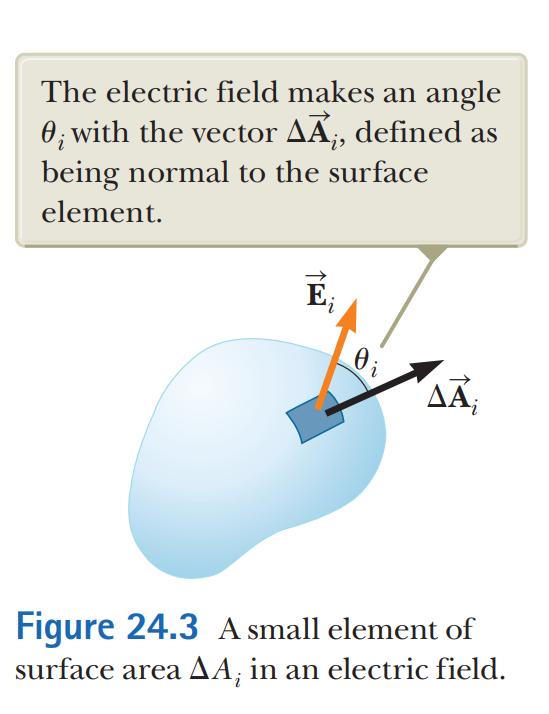
\includegraphics[scale=0.5]{2.PNG}
\end{center}
\end{wrapfigure}
\\

The net flux is proportional to the number of field lines entering and leaving the surface. 
\begin{align*}
`\Phi_E \propto l_{leaving}-l_{entering}
\end{align*}

\noindent An Integral over a closed surface becomes,
\begin{align*}
\Phi_E = \oint \vec{E}\cdot d\vec{A}
\end{align*}

If there exists no charge inside, and the surface is closed, the electric flux is always zero. As the number of field lines entering is the same number of field lines leaving.
\newpage
\section*{24.2 Gauss Law}

\begin{wrapfigure}{r}{0.3\textwidth}
	\begin{center}
		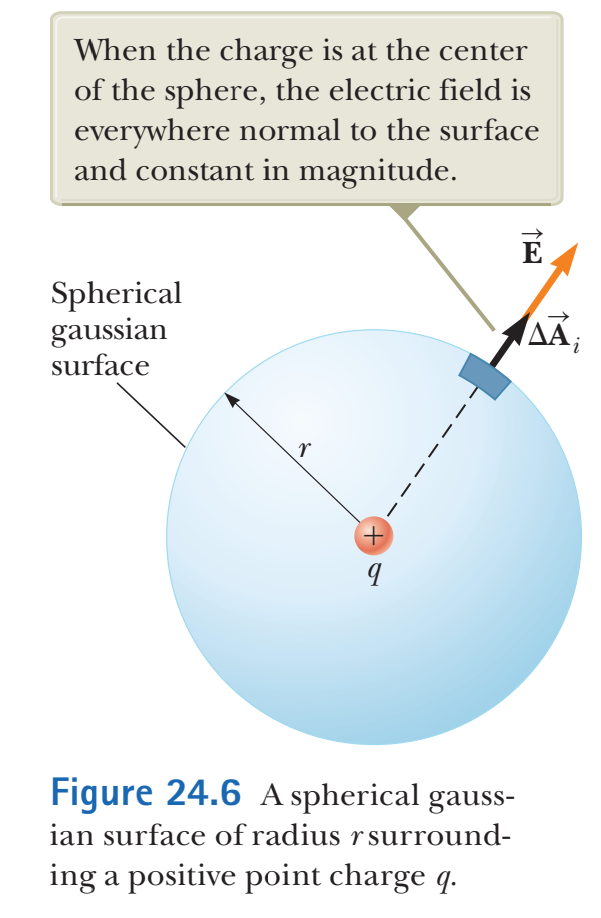
\includegraphics[scale=0.5]{3.PNG}
	\end{center}
\end{wrapfigure}



Assume a point charge at $+q$ inside a closed surface (sphere) of radius $r$. Since the field lines from the positive charge are going to be perpendicular to the surface, and therefore are also going to be parallel to the surface of our sphere. (Parallel to $\vec{A}$). 

We can rewrite the equation more simply as,
\begin{align*}
	\Phi_E = \oint \vec{E} \cdot d\vec{A} = \oint E dA = E \oint dA
\end{align*}
The surface area of a sphere is given as, 
\begin{align*}
A = 4\pi r^2
\end{align*}
Plugging that in for our A when we integrate,
\begin{align*}
\Phi_E = E (4 \pi r^2) = k_e \frac{q}{r^2}(4\pi r^2) = 4\pi k_e q
\end{align*}
We however know from previous chapters that $k_e = 1/4\pi \epsilon_0$
\begin{align*}
	\Phi_E = \frac{1}{4\pi \epsilon_0}4\pi q
\end{align*} 
Simplifying, we the get,\\

\noindent\fbox{%
	\parbox{\textwidth}{%
		\textbf{Gauss' Law}
	\begin{align}
		\Phi_E = \frac{q}{\epsilon_0}
	\end{align}	
	The net flux for any Gaussian Surface (closed surface) surrounding a point charge $q$ is given by $q/\epsilon_0$ and in independent of the shape of that surface
}
}
\begin{wrapfigure}[12]{r}{0.5\textwidth}
	\begin{center}
		\vspace{-0.5cm}
		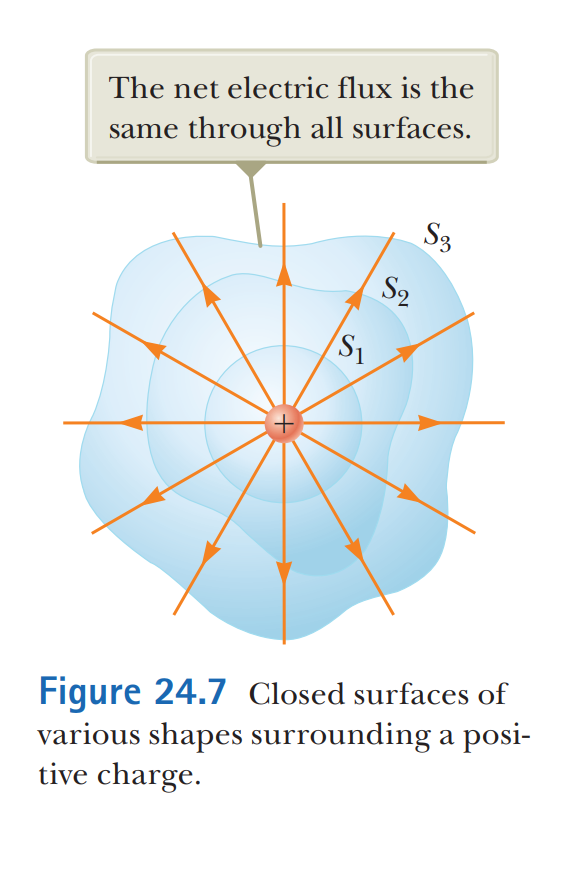
\includegraphics[scale=0.5]{4.PNG}
	\end{center}
\end{wrapfigure}
\\

\noindent But note that,
\begin{align*}
	\oint \vec{E}\cdot d\vec{A} = \oint (\vec{E_1}+\vec{E_2}+...)\cdot d \vec{A}
\end{align*}
So instead, we can generalize this to all charges inside the closed surface,
\begin{align*}
\Phi_E = \oint \vec{E} \cdot d\vec{A} = \frac{q_{inside}}{\epsilon_0}
\end{align*}
Where $q_{inside} = q_1 + q_2 + ... + q_n$ for all n charges inside the closed surface
\newpage
\section*{24.3 Applications of Gauss' Law}
\begin{align*}
\Phi_E = \vec{E} \cdot d\vec{A}
\end{align*}
\begin{enumerate}
	\item The value of the electric field can be argued by symmetry to be constant over the portion of the surface
	\item The dot product can be simplified to simple multiplication of $E dA$ if the vectors are parallel
	\item The The dot product is zero if the vectors are perpendicular such that $\theta = 90^{\circ}$
	\item The electric field is zero over the portion of the surface
\end{enumerate}
The goal in this unit is to find the simplest closed surface to enclose your object inside. Such that the field vectors would be parallel to E and everything else would cancel.\\

\noindent Surface Examples include, how to find the electric field, given surfaces such as,
\begin{center}
	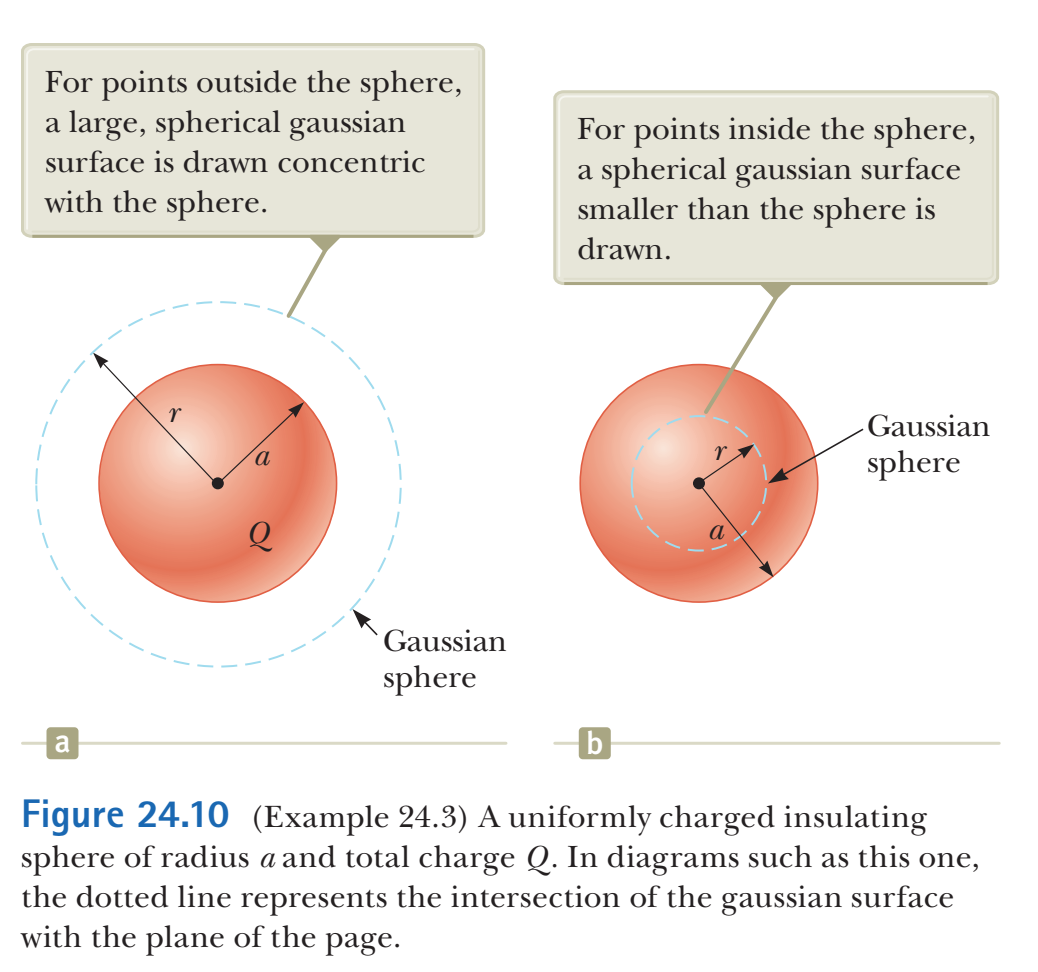
\includegraphics[scale=0.4]{5.PNG}
	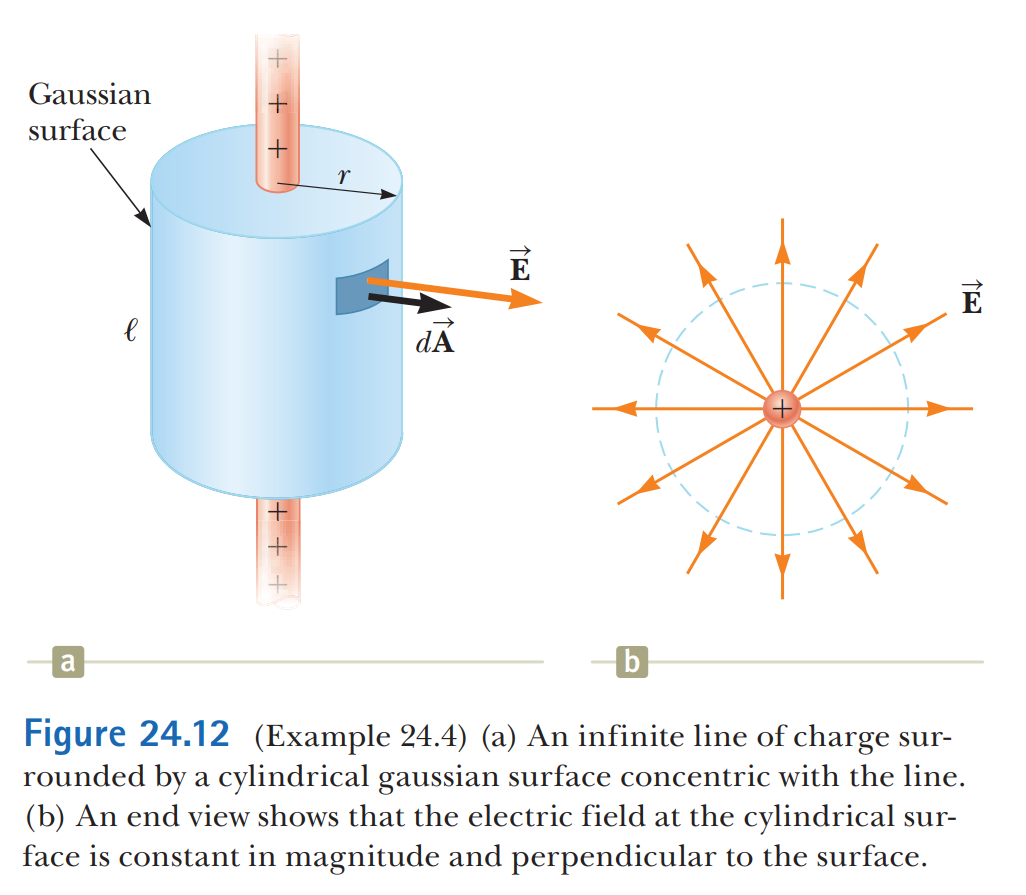
\includegraphics[scale=0.4]{6.PNG}
	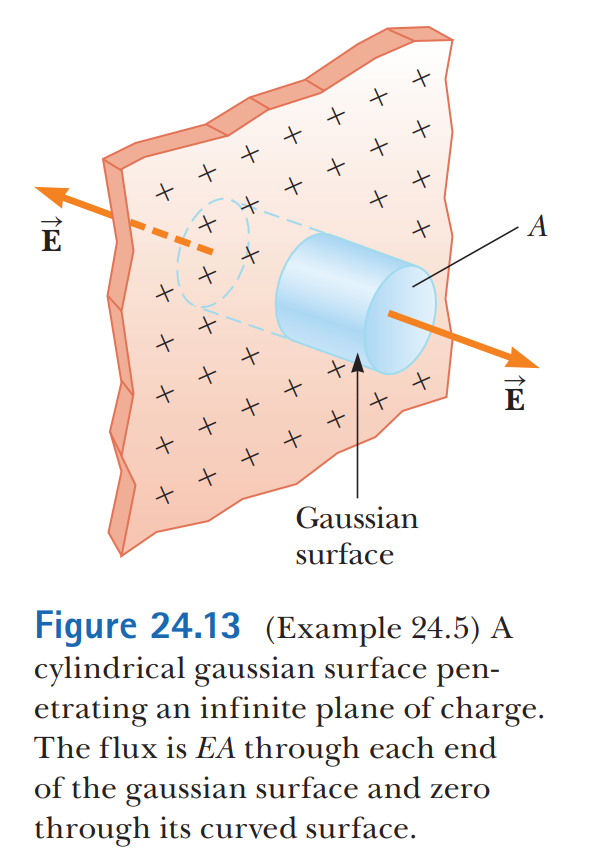
\includegraphics[scale=0.5]{7.PNG}
\end{center}
\newpage 
\section*{24.4 Conductors in Electrostatic Equilibrium}
\noindent\fbox{%
	\parbox{\textwidth}{%
		\noindent When there is no net movement of charge within a conductor, the conductor is said to be in \textbf{electrostatic equilibrium}. A conductor in electrostatic equilibrium has the following properties:
\begin{enumerate}
	\item The electric field is zero everywhere inside the conductor, whether the conductor is solid or hollow.
	\item If the conductor is isolated and carries a charge, the charge resides on the surface.
	\item The electric field at a point on the outside a charged conductor is perpendicular to the surface of the conductor and has a magnitude of $\sigma/\epsilon_0$, wher`e $\sigma$ is the suface charge density at that point.
	\item On an irregularly shaped object, the surface charge density is greatest at locations where the curvature is the smallest.
\end{enumerate}
}}\\

\noindent
\begin{wrapfigure}{r}{0.3\textwidth}
	\begin{center}
		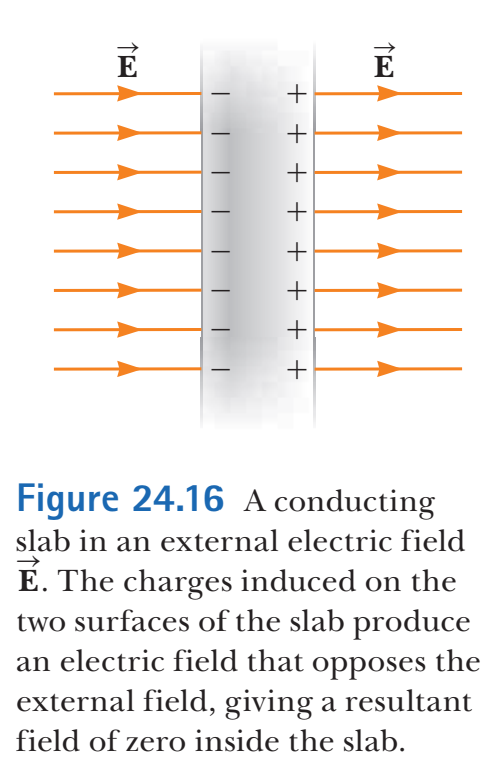
\includegraphics[scale=0.5]{8.PNG}
	\end{center}
\end{wrapfigure}
Notice in this figure, when an external field is applied, electrons accelerate against the field moving towards the left of the slab. Positively charged particles move in the direction of the field and therefore gathering at the right side of the slab. This causes there to be an electric field inside the conductor which opposes the external field. Given enough time, the inner field will get strong enough such that the net field is zero. 
\\

\noindent Since there is no net field inside a charged conductor, any net charges must reside on the surface of the conductor. 
\\

\noindent Since the conductor is electrostatic equilibrium, the $\vec{E}$ has to be perpendicular to the surface as to not move charges inside the conductor. Therefore, we can simply use the algebraic version referring to 24.3 point 2. 
\begin{wrapfigure}{r}{0.3\textwidth}
	\begin{center}
		\vspace{-2.5cm}
		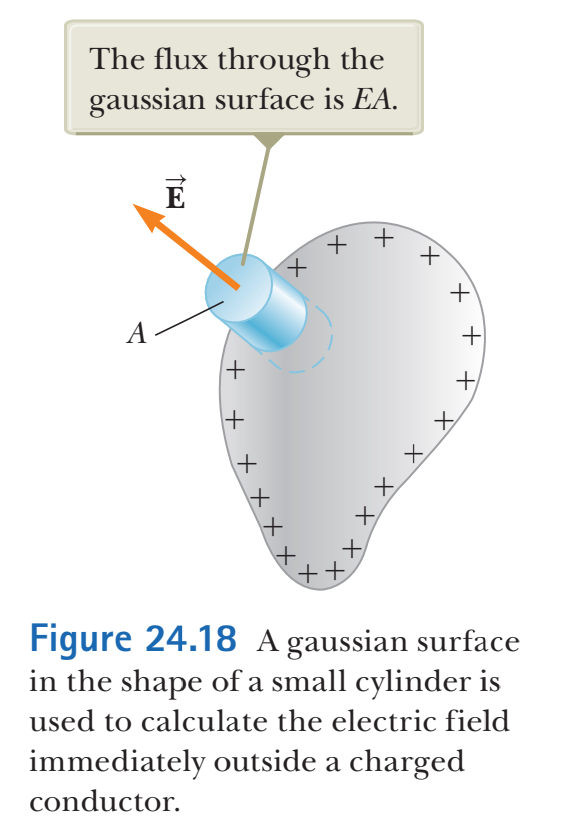
\includegraphics[scale=0.5]{9.PNG}
	\end{center}
\end{wrapfigure}
\begin{align*}
\Phi_E = \oint EdA = EA = \frac{q_{inside}}{\epsilon_0} = \frac{\sigma A}{\epsilon_0}
\end{align*}

Therefore, the electric field at the surface of a conductor is,

\begin{align*}
	E = \frac{\sigma}{\epsilon_0}
\end{align*}

\noindent
When we took the surface integral on the previous page we found only the net charge due to the charges on the surface

\end{document}